\documentclass[a4paper,12pt,fleqn]{report}

%
% PACKAGES %
%
\usepackage[utf8]{inputenc}
\usepackage[export]{adjustbox} % loads also graphicx
\usepackage{natbib}	% harvard ref 
\usepackage{epsf}
\usepackage{psfig}
\usepackage[font={small,it}, justification=centering]{caption}
\usepackage{multirow}
\usepackage{makecell}
\usepackage{amsmath,mathtools}	% maths 
\usepackage{hyperref}	% linked references 
\usepackage[nottoc,numbib]{tocbibind}
\usepackage{listings}	% code
\usepackage{parcolumns}	% columns
\usepackage[toc, acronym, nonumberlist]{glossaries}
\usepackage{dirtytalk} % cites in-text
\usepackage{amssymb} % symbols (check)
\usepackage{pifont} % symbols (cross)
\usepackage{colortbl,xcolor} 
\usepackage[toc,page]{appendix}
\usepackage{multicol} 
\usepackage{chngpage} % change page attr ad-hoc	
\usepackage{float} % position of floats in the doc
\usepackage{array} % tables attributes

%\usepackage{enumitem,amssymb}	% checked lists
%\usepackage{pifont}	% checked lists



%
% CONFIGURATION 
%
\graphicspath{ {imgs/} }
\def \chapterspath {./chapters}
\makeglossaries
\loadglsentries{glossary}
\glsaddall

\def \uncheckedbox {\hspace{0.1cm} \makebox[0pt][l]{$\square$} \hspace{0.3cm}}
\def \checkedbox {\hspace{0.1cm} \makebox[0pt][l]{$\square$}\raisebox{.15ex}{\hspace{0.1em}$\checkmark$} \hspace{-0.1cm}}

\newcommand{\xmark}{\ding{55}}%
\newcommand{\realblankpage}{\newpage\thispagestyle{empty}\mbox{}}

\newcolumntype{L}[1]{>{\raggedright\let\newline\\\arraybackslash\hspace{0pt}}m{#1}}
\newcolumntype{C}[1]{>{\centering\let\newline\\\arraybackslash\hspace{0pt}}m{#1}}
\newcolumntype{R}[1]{>{\raggedleft\let\newline\\\arraybackslash\hspace{0pt}}m{#1}}

%\renewcommand{\bibname}{References}



% checked lists
% --------------
%\newlist{levels}{itemize}{2}
%\setlist[levels]{label=$\square$}
%\newcommand{\cmark}{\ding{51}}%
%\newcommand{\xmark}{\ding{55}}%
%\newcommand{\done}{\rlap{$\square$}{\raisebox{2pt}{\large\hspace{1pt}\cmark}} \hspace{-2.5pt}}
%\newcommand{\wontfix}{\rlap{$\square$}{\large\hspace{1pt}\xmark}}


%
% TITLE
%
\title{
	{Intelligent Assistant with Face Recognition}\\
	\vspace{0.9cm}
	\begin{adjustwidth}{-2cm}{-2cm}
		\centering
		\begin{tabular}{l r}
			\\
			\multicolumn{1}{c}{{\large University of Limerick}}  & \multicolumn{1}{c}{{\large University Carlos III of Madrid}} \\
			{
\includegraphics[width=7cm]{frontpage/ul_logo.jpg}} & {
\includegraphics[width=7cm]{frontpage/uc3m_logo.jpg}}
		\end{tabular}	
	\end{adjustwidth}
	%\vspace{0.8cm}
}
\author{
	\textbf{Erasmus Student:} Mario Sánchez García\\
	UL Student ID: 17150868 \hspace{1cm} UC3M Student ID: 100315075\\
	\\
			\textbf{Supervisor:} JJ. Collins\\
	\\
			CS4617/8 - Computer Systems Project 1/2
}
				\date{April 20, 2018}


%
% FORMAT %
%
\linespread{1.3}    
\pagestyle{plain}

\setlength{\textheight}{8.5in}
%\setlength{\oddsidemargin}{0.7in}
%\setlength{\evensidemargin}{0.7in}
\setlength{\textwidth}{5.50in}
\setlength{\topmargin}{0.0in}
\setlength{\headheight}{0in}
\setlength{\headsep}{0in}
\setlength{\parindent}{12mm} % paragraph indent
%\setlength{\parindent}{0pt}
\setlength{\parskip}{1ex plus 0.5ex minus 0.2ex} % spacing between paragraphs

%%%%%%%%%%%%%%%%%%%%%%%%%%%%%%%%%%%%%%%%%%%%%%%%%%%%%%%%%%%%%%%%%%%%%%%%%%%%%%%

\begin{document}

\pagenumbering{gobble}

\maketitle
\vfill

\realblankpage

\begin{abstract}

The aim of this project is to design and implement an \textit{Intelligent Assistant}, whose objective will be to recognise and identify the face of a student in order to provide personalised support. This support will consist on showing the timetable of the student and the route for their next class. The target of this project are students who have recently come to the University of Limerick, mainly Erasmus students. There are multiple approaches on how to develop face recognition, but in this case we have chosen Convolutional Neural Networks, as they are currently the state-of-art in face recognition, and in order to work with them, we are going to use the open source library \textit{TensorFlow}. \\
\\
However, the calculations done by this library need a computer with a certain power and therefore a considerable size. To provide mobility to the intelligent assistant and achieve a lightweight structure, the system is divided in two independent applications. First, a small, low-cost and basic computer named \textit{Raspberry Pi}, is going to be used to get the data from the camera and act as the user interface. This Raspberry will communicate as a client with the second part of the application: a Flask Server, allocated in another machine with higher specs. In this machine, we will use the data captured by the camera and the TensorFlow library to procced with the facial recognition and, in the final stage, to find the timetable of the student and the route to their next class. 

\end{abstract}













\realblankpage

\section*{Acknowledgements}
\label{cheers}
After finishing this Final Year Project (FYP), I feel the need to look back and thank all the people that have helped and supported me during all this time. 

First I must thank my family, and specially my parents. For their attempt to understand endless nights (sometimes literally) confined with my computer to finish projects, assignments and deliveries. They will never cease to impress me with their infinite patience and unconditional support. Either with calls or in person, which has been a bit difficult lately, they have been always there to give me a pat on the back and say "You can do it". I must apologise with my parents, who came explicitly to Ireland to see me and I could not be all the time I wanted with them because of this project, and my own errors. I love you all and I thank you for the opportunity you gave me with my degree and this Erasmus.

To J.J. Collins, my supervisor and Erasmus coordinator in the University of Limerick. He has helped and guided me throughout all this project. Besides, he accepted my request of doing this FYP here, when I know it is not usual to do it abroad and it could have meant more work for him. For letting me know that "Working like a dog" is the only way things like this FYP are actually possible.

To all my classmates of the UC3M in general, and to my crazy group of friends in particular. For those talks before the exam to revise everything, from where I always learn something that was going to be in the exam, for those talks after to argue about "No, but I answered...", for those days and nights in the laboratories doing assignments. But also for laughing of everything, every time and no matter what, for making the University much easier just by being there. I thank you Luis, Jose and Juan for these four years. I want to thank Juan specially, for his direct support with this FYP, helping me to find the old notes from the second and third year (who could know they were going to be useful again), coming late to his swimming lessons because we were talking on Skype. \\
\\
To all the UC3M professors, because your passion for teaching inspired me and made me love this degree and the Carlos III University itself. Despite all the projects, exams and submissions that I once hated, I know I will miss these last 4 years.

To all the friends from my home town, Perales de Tajuña, and surroundings. You took me out of my house when an assignment was too hard, too long, too difficult. You just invited me to watch a movie, to talk about anything, to play some video games. Coming back home, the assignment suddenly was not that difficult, that long, that hard. It even seemed like it could be done. Thanks for being always there to get me a smile and, knowing it or not, for helping me in the process.

And last but not least, to the new friends I have made in my Erasmus in Ireland. When we came here 9 months looked like a lot of time, but now we are at the end of this experience and I cannot say any other thing than thanks. Being away from home has been difficult, but it would have been unbearable without friends. Thanks specially to my roomate Gautier, for the pizza nights, for the Gravity Falls episodes we watched every time we needed a break and for being a great friend that I will not forget.

Thanks to you all. 

\realblankpage
\pagenumbering{roman}
\setcounter{page}{6}

%
% Table of Contents
%
\tableofcontents

%
% List of Figures
%
\listoffigures

%
% List of Tables
%
\listoftables

%
% Glossary of terms
%
\printglossary[title=Glossary of Terms, toctitle=Glossary of Terms]
\printglossary[type=\acronymtype]
\clearpage
\pagenumbering{arabic}

\chapter{Introduction}
\label{introduction}


\section{General Introduction}
Humans have used body characteristics such as face, voice or even gait to recognize each other for thousands of years. In the mid-19th century, Alphonse Bertillon (chief of the criminal identification division of the police department in Paris, France) developed and then practised the idea of using body measurements to identify criminals. In the late 19th century, the idea of Bertillon lost popularity due to the far more practical discovery of the distinctiveness of human fingerprints (\cite{jain_biometrics}). 

Nowadays, biometrics have advanced to the point that it is no surprise if criminals are imprisoned because their fingerprints were found in the crime scene. However, other biometric methods are not as known as fingerprints and for certain people it is something that can only be found in science fiction movies. Their doubts are not unfounded, biometrics have long been used in science fiction movies to portray futuristic worlds of advanced technology. From retina scans to voice identification and facial recognition, these technologies have been seen on the big screen for more than 50 years (\cite{biometrics_in_scifi}). 

Nonetheless, as we can see in \cite{iphonex_and_other_uses}, face recognition is already being used around the world to examine, investigate, and monitor. There it is explained how in the United States, more than half of all American adults are in a face recognition database that can be used for criminal investigations, simply because they have a driver’s license. In the UK, face recognition was also used at an annual West Indian cultural festival to identify revelers in real-time. 

Although biometrics, and therefore face recognition, emerged from its extensive use in law enforcement to identify criminals, it is being increasingly used today to establish person recognition in a large number of civilian applications (\cite{jain_biometrics}), such as the recently released FaceID for the new iPhone model that identify the face of the owner to unlock the phone. 

The technology around face recognition has advanced following diverse paths, being neural networks the most recent and successful. Within neural networks, there is one particular type of deep, feedforward network that was much easier to train and generalized much better than networks with full connectivity between adjacent layers. This was the \gls{cnn}. It has achieved many practical successes during the period when neural networks were out of favour and it has recently been widely adopted by the computer-vision community (\cite{lecun2015deep}). 

With the advent of several open source libraries, face recognition is now possible and available for everyone. Among this motley group of open source libraries, we find Tensorflow, originally developed by the Google Brain team for the purposes of conducting \gls{ml} and deep neural networks research (\cite{tensorflow_main_website}). Despite the fact that before TensorFlow there were plenty of \gls{ml} libraries that offered great functionality and were reasonably well documented (e.g. \cite{theano_main_site}, \cite{caffe_main_site}), this library has become very popular in the last years thanks to its powerful yet easily readable API, written in Python. 

These such libraries would not be possible without the previous work done in the fields of \gls{ml}, \gls{ai} and face recognition by researchers like Yann LeCun, Yoshua Bengio or Geoffrey Hinton (\cite{rumelhart1985learning}, \cite{lecun1995convolutional}, \cite{lecun1998efficient}, \cite{lecun1998gradient}, \cite{bengio2009learning}, \cite{krizhevsky2012deep}, \cite{lecun2015deep}), and it will be further discussed in the following sections.

In this report we will explain the development of an application that we have called \textit{Intelligent Asissistant}. It is based in one of the currently most advanced implementations of face recognition: FaceNet (\cite{facenet_article}), heavily inspired by the previous OpenFace (\cite{amos2016openface}). Here we will use Tensorflow to re-train a kind of \gls{cnn} named \textit{Resnet Inception v1} from one of the models that FaceNet has left available in their Github website (\cite{facenet_github}).

The objective of the \textit{Intelligent Assistant} is to help the students of the University of Limerick in their first days around the University. This help consists in showing them which is the next class that they will have in the day and the path to the classroom. Face recognition is used here to confirm the identity of a student and be able to search the timetable of such student. Other identification approaches were also available, but as a biometric system, face recognition allow students to be identified by "who they are", rather than "what they possess" (e.g. student ID card) or "what they remember" (e.g. password), which may be things not very clear in the first caotic days in the University. 

The timetable information can be publicly accessed, in the website \textit{timetable.ul.ie}, so applying a technique known as web \gls{scraping}, the student's timetable is obtained and then analysed in order to find their next class. The path to the next class will be shown as a Google Map image, using the Static Google Map API (\cite{google_maps_static}). The face recognition process is preceded by a face \textit{detection} process, that will crop the face out of the image, removing the background and making easier the identification.

Architecturally, the \textit{Intelligent Assistant} is divided in a laptop, which will run the server that actually perform the different tasks of the assistant, and a small, low-cost and basic computer called Raspberry Pi, which will run the \gls{gui} used to interact with the application and will communicate with the server to obtain the needed information. The whole application is written in Python, allowing us to use the Tensorflow library and to learn this popular language, which, as the topics of \gls{ai} and \gls{ml}, was not previously taught in the study program. 

%\section{Technologies Used}	
%
%	\subsection{Why TensorFlow?}
%	We have talked about TensorFlow as it would be the only library available, but there are many more, some of them even written also in Pyhton . That said, why choose it instead other deep learning library? First, TensorFlow is one of the newest libraries at the moment of writing for deep learning in Python and we want this project to deal with a current issue. And second, this library has two APIs (\cite{tensorflow_main_website}): a high level API (MNIST), which makes it accessible for everyone and it will be easy to start with; and a low level API (Deep MNIST), which can provide a more advanced control for the final development of the project.
%
%	\subsection{Why Raspberry Pi?}
%	TensorFlow still needs a computer with a certain computing power, which also means that it will have a considerable size. In order to provide mobility to the assistant, a client-server architecture is going to be used. In the server side is where face recognition and high computing requirement tasks are actually going to be executed, while the client side will act as the interface of the system. 
%
%	As the client side will not require much computing power, Raspberry Pi becomes an option. With the size of a credit card, Raspberry Pi is a low-cost and barebones computer capable to work as a traditional desktop tower. Many versions of this board have been released, but for this project we have chosen the Raspberry Pi 3 Model B.
%
%	\begin{figure}[ht]
%		\centering
%		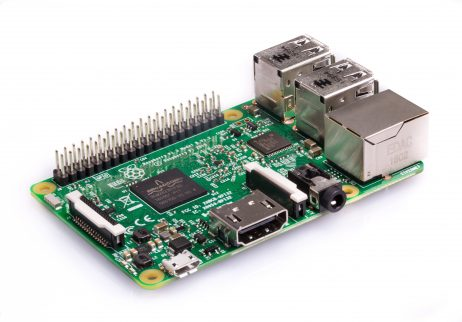
\includegraphics{raspberry-pi-3-b.jpg}
%		\caption{Raspberry Pi 3, model B}
%	\end{figure}
%
%	\subsection{Why Python?}
%	The reasons that made Python the language chosen for this project were many. First, it is the language that Tensorflow uses to express the model of the network, so it was necessary to use it at least for the face recognition module of the project. Second, Python has become a widely used language because (\cite{why_python}):
%
%	\begin{itemize}
%		\item Proven language. Python is used by many important companies, such as Dropbox, Google or Amazon. 
%		\item Fast prototypes. Python's dynamic nature and simple syntax make it perfect for prototyping, preventing us from worrying about the actual implementation and helping to focus on data and algorithms, which the main task of machine learning.
%		\item For everyone. Many data scientist and engineers have a background in maths and statistics, but they may not have any experience in programming. Python's simplicity and readability, as it is said to have a math-like syntax, make it easier to pick up.
%		\item Mature Data Science Ecosystem. There is a great collection of math and data science for Python, incremented by new libraries that are built on top of the older ones (but controlled by the solid Python's packaging). 
%	\end{itemize}
%
%	Finally, the last reason is personal. During the last years in my home University, I heard many times how important Python was and how popular it was becoming. However, the modules from my study program never used this language for their assignments, so I never had the opportunity to learn it in an academic environment. Because of that, I decided to use Python in all aspects of this project in order to learn how to work with it.  

\section{Objectives}
The objectives of this project are many and can be divided in personal and technical. The first and more important personal one is to learn about the fields of Computer Science with which I never experimented before. In my home University (Carlos III of Madrid), I chose the computer architecture specialization in my third year. This means that my knowledge about \gls{ai} and \gls{ml} was almost not existent, as it was taught in the other specializations. 

The situation with the Python language at the beginning of the year was similar, even when it is a well known language and has become very popular in the last years. The modules from my study program never used this language for the assignments, so I never had the opportunity to learn it in an academic environment. Because of that, when my coordinator explained me that for the Tensorflow library I would need to use Python, I decided to use it. Not only in the interaction with the library, but also in the server communication and the application \gls{gui}.

On the other hand, among the technical objectives of this project we can find:
\begin{itemize}
	\item Create a tool called \textit{Intelligent Assistant} to help the students of the University of Limerick to find their next class.
	\item Use Python for the development of this tool.
	\item Divide the system in a client-server communication in order to achieve a light-weight application in the client side.
	\item Use the microframework Flask (never used before either), also written in Python, to create the server.
	\item Use a Raspberry Pi in the client side to act as interface with the students.
	\item Design a graphical user interface that allows to use all the features of the application.
	\item Perform face recognition using the Tensorflow library to identify the students.
	\item Show in the final stage a map with the path from the current position to the location of the next class.
\end{itemize}

\section{Motivation}
This \gls{fyp} was motivated for many reasons that started with the idea of doing it abroad. In my third year I decided to do my fourth and final year of the degree as an Erasmus student, but it was too late to be included in the Erasmus lists of that year. The only option to be able to go on Erasmus was to finish my degree one year later, so I splitted the modules of the fourth year in two groups with the idea of doing the first half of the modules in my fourth year in Spain, and the other half abroad. 

Althought it was forced by the circumstances, I do not regret the fact of doing my \gls{fyp} abroad. It gave me the opportunity to improve my academic writting in English by doing this document, reaching a total of X pages and becoming the longest document I have ever written in English. I must apologise about this fact, because English is not my mother tongue and, even when I have spent much time looking for grammatical errors, there may still be some that I could not detect.

Another motivation of this project, already mentioned in the previous section, was to learn about topics that my degree in Spain did not cover in its study program. The decission I took in my third year of choosing the \textit{computer architecture} specialization closed me the doors to learn about \gls{ai} and \gls{ml}, so this project was the perfect occasion to expand my knowledge on such topics. Besides, other related (e.g. face detection, face recognition) and not related (e.g. Python, web \gls{scraping}, \gls{gui} design) issues that were never treated before, were also included in the project in order to learn more about them. 

\section{Structure of the Document}
This present document is divided in:

\begin{itemize}
	\item Glossary of Terms and Acronyms. List of definitions of the terms and acronyms that have been used in this report and that may result confusing for the reader. Every term and acronym used in the text is linked its definition here.
	\item Introduction. This section, in which we are currently in, includes a little background about biometrics and \gls{ml}, along with a brief explanation of the project and the reasons that motivated its realization.  
	\item Research. In this section, the state of the art of the different fields with which this project is related (i.e. machine learning, neural networks, face detection and face recognition) and some of the technologies used, are widely explained, referencing the books and papers from where the factual information actually comes from. 
	\item Design and Implementation. The complete development process of the \textit{Intelligent Assistant} application can be found here.
	\item Empirical Studies. A total of two empirical studies are included in this section, treating the effectiveness of the approaches used in the project for the face detection (i.e. Viola-Jones Haar cascades) and the face recognition (i.e. \glspl{cnn}).
	\item Discussion and Conclussion.
	\item Appendices. 
	\begin{itemize}
		\item Appendix A. Set of icons used in the \gls{gui} of the application.
		\item Appendix B. Actual captures of the final version of the \gls{gui} of the application.
	\end{itemize}
\end{itemize}




\chapter{Research}
\label{research}

%\section{Introduction to Machine Learning}			
%\section{Artificial Neural Networks}				
%\section{ANNs vs CNNs} 					% disabled for now
%\section{The Perceptron}
%	\subsection{Linearly Separable attribute}		** (img)
%	\subsection{Training Rule}
%	\subsection{Delta Rule and Gradient Descent}
%	\subsection{Derivation of Gradient Descent}
%	\subsection{Gradient Descent Algorithm}
%	\subsection{Stochastic Approximation}
%\section{Multilayer Perceptron Networks}
%	\subsection{Is a perceptron valid for MLP? The Sigmoid Unit}
%	\subsection{Backpropagation Algorithm}
%\section{Face Recognition using CNNs}		% disabled for now
%\section{Voice Recognition}				% disabled for now
%\section{Public Data Sets}
%\section{Raspberry Pi}											*new*
%	\subsection{Using the Pi-camera}							*new*
%\section{Python}
%	\subsection{Threads}										*new*
%	\subsection{Synchronization}								*new*		

\section{Introduction to Machine Learning}
Machine learning is a term difficult to define, it can be seen from many points of view: it could be Data Mining (applied to databases), Inference (Statistics) or Pattern Recognition (Engineering). One clear thing is that machine learning is a field of artificial intelligence that studies systems that can learn from data. As Kevin P. Murphy said, "The goal of machine learning is to develop methods that can automatically detect patterns in data, and then to use the uncovered patterns to predict future data or other outcomes of interest". 

Within machine learning we can find two different approaches: supervised or unsupervised learning. If you suppose you are providing solution to your kids for each and every situation in their life, it is called they are supervised. But, if your kids take their decisions out of their own understanding, it is called they are unsupervised . Well, something similar happens with machine learning. If you train your model for every input with a corresponding target, then it is supersived learning (you give extra information apart from the data itself) and it will be able to provide target for any new input after sufficient training. Contrary, if you train your model with only a set of inputs it is unsupervised learning and it will be able to find relationships between the different inputs (\cite{sup_unsup_learning}). 

\section{Artificial Neural Networks}
Artificial Neural Networks (ANN) have generated a lot of excitement in Machine Learning research and industry, thanks to many breakthrough results in speech recognition, computer vision and text processing. It is a computational model that is inspired by the way biological neural networks in the human brain process information (\cite{intro_ann}). 

ANN are based in singular units of computation, called neurons, nodes or simplyly units. It receives input from some other nodes, or from an external source and computes an output. Each input has an associated weight ($w$), which is assigned depending of its relative importance to other inputs. The node applies a function $f$ to the weighted sum of its inputs, as we can see in the next figure (\cite{intro_ann}).

\begin{figure}[ht]
	\centering
	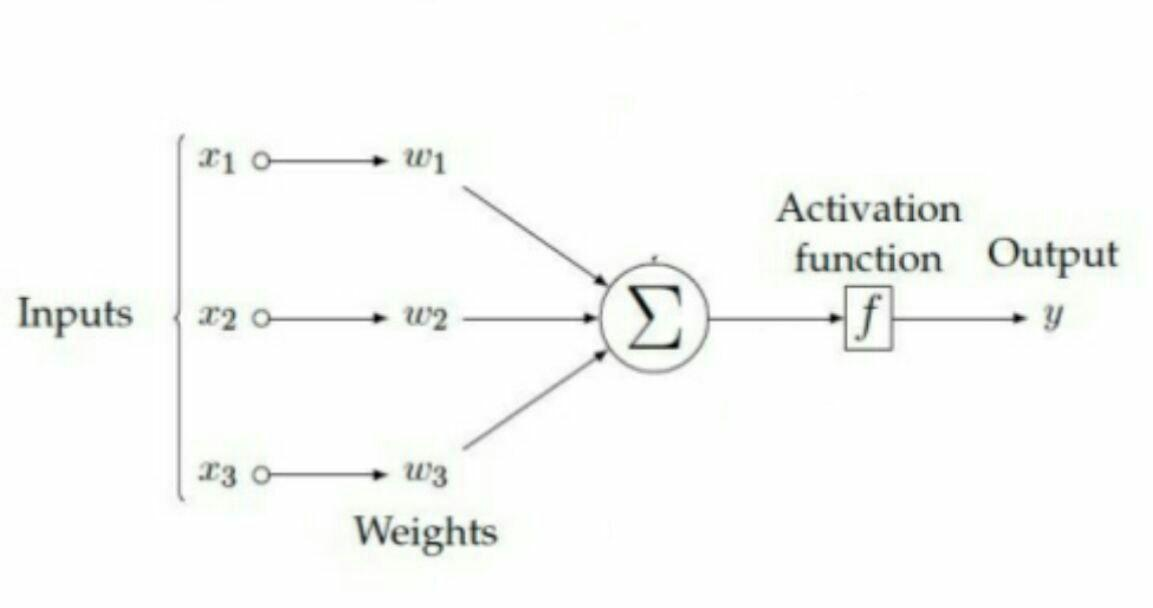
\includegraphics[width=\textwidth]{neuron.jpg}
	\caption{Neuron model}
\end{figure}

These neurons are arranged in layers to construct an ANN. Nodes from adjacent layers have connections between them, so each connection has associated a weight. Because of the position of these nodes and the connections between them we can differentiate three types of nodes: input, hidden and output nodes. 

\begin{figure}[ht]
	\centering
	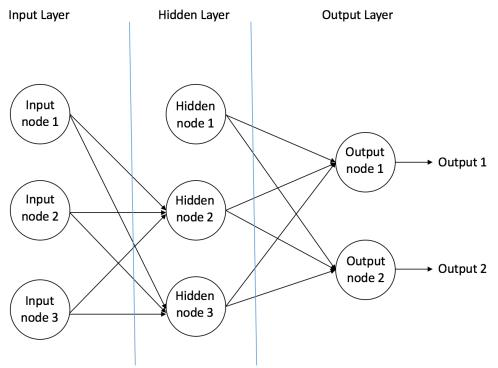
\includegraphics[width=\textwidth]{ann_basic_model.jpg}
	\caption{Basic Artificial Neural Network}
\end{figure}

\begin{itemize}
	\item Input Nodes. Provide information from the outside world without computing anything, they just past the information to the hidden nodes. Together are referred to as the \textit{Input Layer}. 
	\item Hidden Nodes. They have no connection with the outside world (hence the name "hidden"), but they compute the information provided from the previous layer and give the output to the next one. Together are referred to as the \textit{Hidden Layer}. Although these networks must have only one input layer and one output layer, they can have more than one hidden layer (or none). 
	\item Output Nodes. Together are referred to as the \textit{Output Layer} and they are responsible to transfer the computed information to the outside world again.
\end{itemize}

\section{The perceptron}
Within the Artificial Neural Networks (ANN), we can find great variety of units that define the type of ANN involved, but in order to explain how they work, we are going to use a perceptron. This unit has several inputs that are used to perform an operation involving all of them, to finally calculate a single value as a result in a single output.

Each input is composed of a value and a weight, which will indicate the contribution that will contribute to the output of the perceptron. The operation involving all inputs is a linear combination:

\begin{equation}
    \label{linear_combination}
        y=\sum_{i=0}^{n} w_n x_n = w_0 + w_1 x_1 + w_2 x_2 + w_3 x_3 + ...%
\end{equation}

where $x_n$ are the inputs of the perceptron and $w_n$ are the weights ($x_0=1$ is not an input, it's an useful constant to allow us to write the linear operation with a summatory). Finally, the (unique) output of the perceptron depends on the result of the linear operation, being 1 if the result is positive; or -1 in another case. All these data allow us to define the perceptron as follows:

\begin{equation}
    \label{perceptron_rule}
	perceptron(y) =
		\begin{cases}
	     	1 & \text{if $y>0$} \\
	        -1 & \text{otherwise} \\
		\end{cases}
\end{equation}

	\subsection{Linearly Separable attribute}
	This atribute refers to the fact that an hyperplane can separate (or not) the different output values of the perceptron, dividing the space in two sides where there is only one kind of output (1 or -1). To explain it better, we are going to use a percetron with two inputs. With this inputs we can produce a Cartesian map (first input would be X axis; and second input, Y axis). Instead of using a point to represent the input, we use the output symbol (``"+``" or ``"-``"). If we can draw a line (our hyperplane in a 2-dimension space) that divides the map in two sides, so that on each side of the line we can only find one kind of symbol (all positives or all negatives), then we can say that the set of points we have used is linearly separable.  
	
	With a single perceptron there are sets of points that can't be linearly separable. That's why networks of perceptrons with more than one layer are created, whose first layer perceptron's outputs is not the final result, but performs the role as input to another perceptron in the next layer. This way, even the non-linear surfaces can be represented.

	\subsection{Training Rule}
	In order to train perceptrons, we begin assigning random values to the weights and then we apply the perceptron to each training example. If the perceptron misclassifies an example, the training rule will modify the weights according to:

	\begin{equation}
		\label{training_rule}
		w_{i}^{'} \leftarrow w_{i} + \eta (t - o) x_{i}
	\end{equation}

	where $\eta$ is the \textit{learning rate} (constant usually small that determines how much weights vary in each step), $t$ is the target value, $o$ is the actual output that we have obtained from the perceptron and $x_{i}$ is the input value.

	The weights will converge to a value that classify correctly within a finite number of iterations if (and only if) examples are linearly separable and the $\eta$ value used is sufficiently small.
	
	\subsection{Delta Rule and Gradient Descent}
	When the input set is not linearly separable, we need an alternative to the training rule: delta rule. Delta rule uses gradient descent to search for the hypothesis space (set of outputs) that best fit the training example. 

	To explain this we’re going to use a linear unit (not thresholded as the perceptron) which output is calculated by $o = \vec{w} \cdot \vec{x}$. To measure the training error we’re going to use the next formula, where $D$ is the set of examples. It depends only of $\vec{w}$ because we assume that its relation with the examples set $\vec{x}$ will be gone after the training.

	\begin{equation}
		\label{error_function_full_square}
		E(\vec{w}) = \frac{1}{2} \sum_{d \varepsilon D} (t_d-o_d)^2 
	\end{equation}

	If error is defined by this formula, its representation (assuming two inputs) would be a parabolic surface with only one local minimum. The gradient descent will start using a random initial vector and the algorithm will modify its direction step by step. In each step, the algorithm will choose the variation that go the deepest along the error surface. By this way, the process will continue until the local (and global minimum in this case) is reached.

	\begin{figure}[ht]
		\centering
		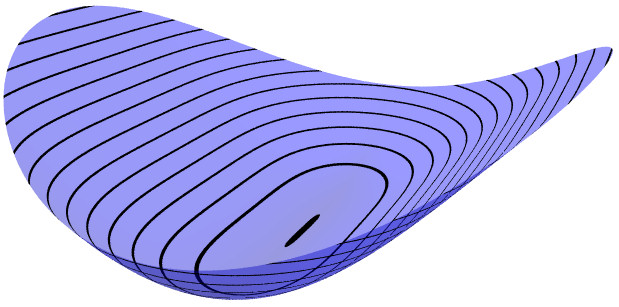
\includegraphics[width=\textwidth-30mm]{parabolic_surface.jpg}
		\caption{Parabolic Surface with one local minimum}
	\end{figure}

	\subsection{Derivation of Gradient Descent}
	To modify the direction of the vector we will derivate the error function ($E(\vec{w})$) respect of $\vec{w}$, form that is called \textit{gradient of E}:

	\begin{equation}
		\label{gradient_of_E}
		\nabla E(\vec{w})= [\frac{\partial{E}}{\partial{w_{0}}}, \frac{\partial{E}}{\partial{w_{1}}}, ..., \frac{\partial{E}}{\partial{w_{n}}}]
	\end{equation}

	This vector specifies the direction that produces the steepest increase in E, so including a negative factor ($-1$) we can calculate the steepest decrease in E. We can represent the training rule with its component form:

	\begin{equation}
		\label{training_rule_component_form}
		w_{i}^{'} \leftarrow w_{i} + \Delta w_{i} \hspace{1.5cm} ; \hspace{1.5cm} \Delta{w_{i}}=-\eta \frac{\partial{E}}{\partial{w_i}}
	\end{equation}

	So the final expression of the gradient descent is:

	\begin{equation}
		\label{gradient_descent_final_expr}
		\Delta w_i = -\eta \frac{\partial{E}}{\partial{w_i}} = \eta \sum_{d \varepsilon D} (t_d - o_d) x_{id}
	\end{equation}


	\subsection{Gradient Descent Algorithm}
	A brief version of the algorithm would be as follows:

	\begin{enumerate}

		\item Pick an initial random weight vector.
		\item Apply the linear unit to all training examples and then compute $\Delta w_i$  using the gradient descent formula.
		\item Update each weight adding $\Delta w_i$.
		\item If the algorithm hasn’t reached the local minimum, repeat from step 2.
	
	\end{enumerate}

	\subsection{Stochastic Approximation}
	Instead of using all the examples to update the weight each step (which could imply a lot of work) there is another option: incremental/stochastic gradient descent. This way we will approximate the gradient descent updating the weights with each training example:

	\begin{equation}
		\label{delta_rule}
		\Delta w_{i}= \eta (t - o) x_{i}
	\end{equation}

	So the error function must be changed to:

	\begin{equation}
		\label{error_function_stoc_square}
		E(\vec{w}) = \frac{1}{2} (t_d-o_d)^2 
	\end{equation}

\section{Multilayer Perceptron Networks}
A single perceptron can only express linear decision surfaces, so it is very limited for real life situations. In contrast, a multilayer network learned by the backpropagation algorithm can express a rich variety of non-linear decision surfaces, which are more suitable for that kind of problems.

	\subsection{Is a perceptron valid for MLP? The Sigmoid Unit}
	A perceptron unit is perfectly valid for a MLP, but its discontinuous threshold output make it not suitable at all for gradient descent. Also, as a linear unit, multiple layers of cascaded units will only produce linear functions. Then, another option is required: a \textbf{sigmoid threshold unit}. This unit works pretty similar to the perceptron, but has another function at the output to perform the threshold, which is called logistic or sigmoid function ($\sigma(y)$).

		\begin{equation}
			\label{sigmoid_function}
			\sigma(y) = \frac{1}{1+e^{-y}}
		\end{equation}

	This function increases monotonically and continuously with its input and is able to map a large input domain to a small range (0, 1) of outputs, reason because is usually called \textit{squashing function}. Finally, being easy derivable make it a really good choice for our task. 


	\subsection{Backpropagation Algorithm}
	The Backpropagation Algorithm learns the weights for a multilayer  network, given a network with a fixed set of units and interconnections. It uses gradient descent to minimize the squared error between the output and its target values of the network:

		\begin{equation}
			\label{squared_error_function_network}
			E(\vec{w}) = \frac{1}{2} \sum_{d \varepsilon D} \sum_{k \varepsilon outputs} (t_{kd}-o_{kd})^2 
		\end{equation}

	As we have changed the error function definition, the error surface will have more than one local minima (not as before with a single perceptron). This means that gradient descent may fail in order to find the global minima and only reach a local minima instead. Anyway, it has been proved to produce excellent results even with this problem.

	The stochastic version of the Backpropagation Algorithm, applied for each training example, would be:

		\begin{enumerate}

			\item Input the values in the network and obtain the output values computing every unit of the network.
			\item For each output unit ($k$), calculate its error term $\delta_k$, which is the usual $(t-o)$ multipied to the derivate of the sigmoid function:
				\begin{equation}
					\label{backpropagation_output_error}
					\delta_k \leftarrow o_k (1 - o_k)(t_k - o_k)
				\end{equation}				

			\item For each hidden unit ($h$), calculate its error term $\delta_h$. This is similar to the output formula, but as we don't have a target value for a hidden unit, we must calculate it summing up the errors of the downstream units weigthing each error by the weight of the connection that links them. 
				\begin{equation}
					\label{backpropagation_hidden_error}
					\delta_h \leftarrow o_h (1 - o_h) \sum_{l \varepsilon downstream} (w_{hl} \delta_i)
				\end{equation}

			\item Update each network weight:
				\begin{equation}
					\label{backpropagation_weight_update}
					w^{'}_{ji} \leftarrow w_{ji} + \Delta w_{ji} \hspace{1.5cm} ; \hspace{1.5cm} \Delta w_{ji} = \eta \delta_j x_{ji}
				\end{equation}

		\end{enumerate} 

%\section{Face Recognition using CNNs}

%\section{Voice Recognition}	% disabled for now

\section{Public Data Sets} 
Face recognition is nothing but another kind of machine learning and as such, it needs to be feeded with data, face images in this case. The problem is that we need a high amount of them, in addition to that each face image has to be different (or the model would only work well with the data we worked with, and not any face, which is our purpose). As we cannot generate this dataset by ourselves, we must look for a public dataset with enough and different face images:

\begin{itemize}
	\item CASIA Webface Database. It is the second largest database of faces (first is private and belongs to Facebook), with more than 10,000 subjects and almost 500,000 images. In order to use it an agreement needs to be signed so the database will only be used for non-comercial, research or educational purposes. We finally discarded it because its size, which would be more suitable for a big project with a research group (\cite{casia_db}). 
	\item WIDER FACE. This database counts with more than 32,000 images and can be freely accessed by a Google or Baidu Drive. It has the advantage that its images are already labelled and the faces in them are marked. However, many of the images have more than one face on them (they say they count with almost 400,000 faces in the dataset) and we need them to have only one person (\cite{widerf_db}).
	\item Labelled Faces in the Wild (LFW). This database only counts with more than 13,000 images that only have one person in them, which is perfect for the scope of this project. It can be explored online and has been recently updated, solving some erratum. Finally, it also has the option to download the images aligned with funneling or commercial software, reducing the work to do on the dataset. Because of all these reasons, it is the dataset that is going to be used for the project (\cite{lfw_db}).
\end{itemize}

\section{Python}
In the Introduction of this project we already have enumerated some of the features of this language, but there is much more. First, it is a high-level language designed to be easily readable. One interesting example of this is the lack of brackets ("{}"), which is the usual way to delimit control flow blocks in other languages. Instead, Python uses indentation, so to indicate a line is inside a function or an \textit{if} block, we just have to indent it one level more. We can see it clearly in the next comparative.

\noindent\begin{minipage}[t]{.45\textwidth}
\begin{lstlisting}[caption=C code,frame=tlrb, language=C]{Name}
void foo(int x)
{
    if (x == 0) {
        bar();
    } else {
        foo2(x + 3);
    }
}
\end{lstlisting}
\end{minipage}\hfill
\begin{minipage}[t]{.45\textwidth}
\begin{lstlisting}[caption=Python code,frame=tlrb, language=Python]{Name}
def foo(x):
    if x == 0:
        bar()
    else:
        foo2(x + 3)
\end{lstlisting}
\end{minipage}

Second, Python is interactive. When we install Python in our computer we can launch it in the terminal and a prompt will show up, allowing us to interact with the interpreter directly to write our programs. Directly related with this feature is that Python is interpreted. This means that it does not need to be compiled before executing (what happens to languages like C, C++ or Lisp), as it is processed by at runtime by the interpreter (\cite{python_overview}). 

And finally, Python is easy to learn. It has fewer keywords than other languages, its strucure is much simpler and the syntax is easily readable with a certain level of English. It is because all of this why it has become very popular in recent years, being used from to start learning programming to advanced investigation projects.

\chapter{Design and Implementation}
\label{design}

%\section{Scenario}
%\section{Requeriments}
%\section{Design and Architecture}
%	\section{Related work}
%		\subsection{Using Pi-camera to stream}
%\section{Implementation}
%\section{Testing}
%\section{Software Quality}

\section{Introduction}
In this section, the design process that has been followed for the implementation of the application is going to be explained. First we find the requirements of the application, among which functional and non-functional requirements have been distinguished. Using these requirements, we explain how is the activity flow of the application. In this section are also included the prototypes and mockups that were used in the design of the \gls{gui}. 

\section{Requirements}

\section{Scenario}
\section{Architecture and Technologies}
\section{Front end}
\section{Back end}	
\section{Testing}
\section{Implementation issues}
\section{Summary of the implementation}
\section{Software Quality}





%\section{Related work}
%This section will include all the work that has been done for the project, but that is finally not included in the final version. For each related work, along with its explanation, we will also find the pros and cons of the solution and the reasons why it has not been included in the final version.
%	\subsection{Using Pi-Camera to stream}
%	As we explained in previous sections, the objective of the project is to capture (and after analyse) a photo of the face of a user, using the camera connected to the Raspberry Pi (Pi-Camera). Due to the limited scope of a Final Year Project, we added some constraints on how the photo should be, like that the face of the user must be centered in the photo or that they must look directly to the camera (in the Figure XX we can see an example of a photo). 
%
%	In order to provide to the users a way to place themselves correctly in front of the camera before the photo is taken, a preview is needed.	This preview must be shown in a screen, so assuming that the Raspberry Pi is not connected to it, we need a way to stream it in real-time to another computer (which will have a screen connected).
%
%	To start the development, we chose to use the code of an already written server that sends via HTTP a pre-recorded video (\cite{mjpeg_server_base_code}). In this project, the author aims to create "virtual cameras" using the format Motion JPEG (MJPEG), which is basically a sequence of JPEG images showed one after another. Until now, it fits perfectly for our Pi-camera, as it is able to capture in JPEG format.
%
%	However, the performance of this method is way worse than its competitor in the Raspberry Pi for video: h.264. Why choose MJPEG then? As we can see in \cite{mjpeg_format_info}, the MJPEG format "is natively supported by the QuickTime Player, the PlayStation console, and web browsers such as Safari, Google Chrome, Mozilla Firefox and Microsoft Edge". The four most used browsers support natively it, what takes away the work of create an application for the client side to show the stream. 
%
%	The GitHub project was designed to send a pre-recorded video, but we need a real-time video, so we changed the code to include the task of capturing the images. To do this task simultaneously with the image sending, we chose to use threads with a producer-consumer paradigm, synchronizing them using semaphores. The thread capturing the images acts as producer, and the one that computes the server is the consumer.    
%
%		\subsubsection{Pros and Cons}
%		Pros:
%		\begin{itemize}
%			\item Video format (MJPEG) is supported by the most used browsers natively.
%			\item This solution does not require the Raspberry Pi to be connected to the screen. 
%		\end{itemize}
%
%		Cons:
%		\begin{itemize}
%			\item The performance of the video format is poor, reaching a mean of 0.5fps after some testing.
%			\item The Raspberry Pi is included in the project to act as the user interface, so we don't need it away from the screen.
%			\item With only one core, the Raspberry Pi does not work well with threads.
%		\end{itemize}
%		
%		\subsubsection{Why is it not included in the final version?}
%		The poor performance of the stream makes difficult to place correctly the face in the camera, not only because of the mean 0.5 fps reached in the tests, but also for the delay that exits since the camera captures the photo until the browser shows it. 

\chapter{Empirical Studies}
\label{ch:empirical-studies}

\section{Introduction}
In this section we include the analysis of two of the techniques used in the project: the Viola-Jones method and the Convolutional Neural Networks. In order to prove their effectiveness we will perform an experiment for each of them. The experiments have been fully documented, including the data set used and the results, which are discussed at the end.

\section{Experiment 1: Effectiveness of Viola-Jones method for Face Detection}
	\subsection{Objective}
	As it was already explained in the Research section (\ref{subsec:face_detec_techniques}), the Viola-Jones method "stands out for performing a high detection rate with a very low false positive rate and it is capable to work in a real time situation". These features have made it widely used in the recent years and it was also the reason why it was finally chosen for this project. 

	In this experiment, we are going to test this affirmation by applying the method to a certain set of images. It will be composed of an equal proportion of face images, near-face images from a human perspective and non-face images. The results will be displayed including the faces that were correctly detected, the faces that were missed (i.e. false negatives) and the images incorrectly classified as having a face, when they did not (i.e. false positives).

	\subsection{Method and parameters}
	The computer used to run the experiment is a laptop Toshiba C50-A-1GU with a 2,40 GHz Intel Processor Core i3-4000M, 8GB 1600MHz RAM memory and Kubuntu 17.10 OS (Linux kernel version 4.13.0-38-generic). The Viola-Jones method  is applied using the OpenCV library as it was done in the \textit{Intelligent Assistant}. In fact, the code used for this experiment (Figure \ref{fig:fd_experiment_code}) is pretty similar to the included in the \textit{face{\_}detection} module, discussed in the Design chapter (\ref{subsec:face_det}).

	\begin{figure}[!ht]
		\centering
		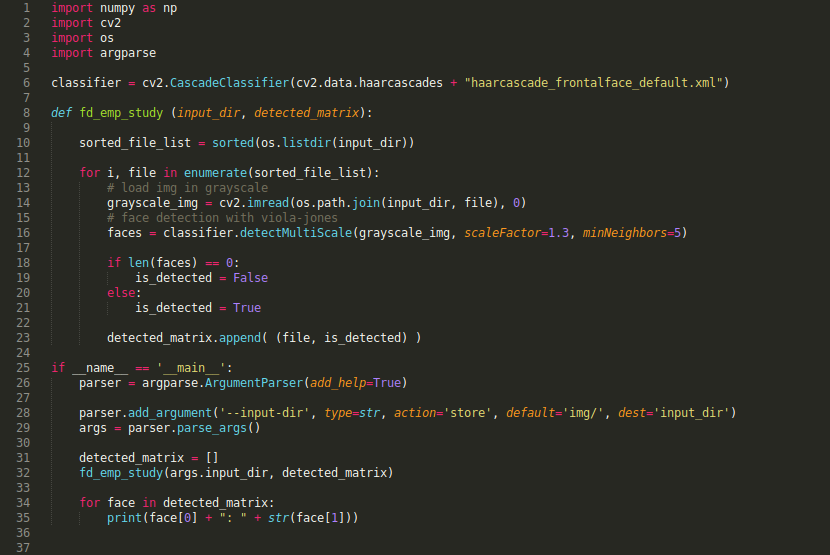
\includegraphics[width=14cm]{emp_studies/fd_experiment_code}
		\caption{Code used to run the Experiment 1}
		\label{fig:fd_experiment_code}
	\end{figure}

	The images are located in a folder named "img", in the same directory as the file. The filename of these images indicates the group to which it belongs and the id of the image, an integer of 2 units filled with zeros if necessary. Then, the filename of the images follow one of these patterns: "face{\_}XX.jpg", "near-face{\_}XX.jpg" or "non-face{\_}XX.jpg".

	The classifier selected for this task is "haarcascade{\_}frontface{\_}default", the same used in the application. The images are loaded in grayscale and the classifier is applied to perform the face detection. This method returns an array with the location of the detected faces in the image, so evaluating its length, we know whether the classifier detected a face or not (i.e. the array would be empty). 

	\subsection{Data set}
	The dataset used in the experiment is composed of a total of 90 images, where 30 of them contain a human face, 30 contain a pattern that humans could interpret as face and 30 do not contain any face. In the Figure \ref we can see the complete dataset. All images are square-shaped with a resolution of 250x250 pixels. The face images belong to the \gls{lfw} dataset (\cite{lfw_db}), while near-face images and non-face images were obtained using Google images and after cropped manually.

	The non-face images were obtained after searching for the keys "background" and "abstract wallpaper". The near-face dataset must be explained in detail because the subjective decission of whether the image look like a face enough or not. This group of photos is internally divided in another three sub-groups:

	\begin{itemize}
		\item Images from 1 to 11. The first contain pencil or graphic drawings that represent persons looking straight forward.
		\item Images from 12 to 20. The second group contain cropped faces from paintings that may have variations in the proportions of some face features. 
		\item Images from 21 to 30. The third and last group contain photos from faces of real sculptures.
	\end{itemize}

	%\begin{figure}[!ht]
	%	\centering
	%	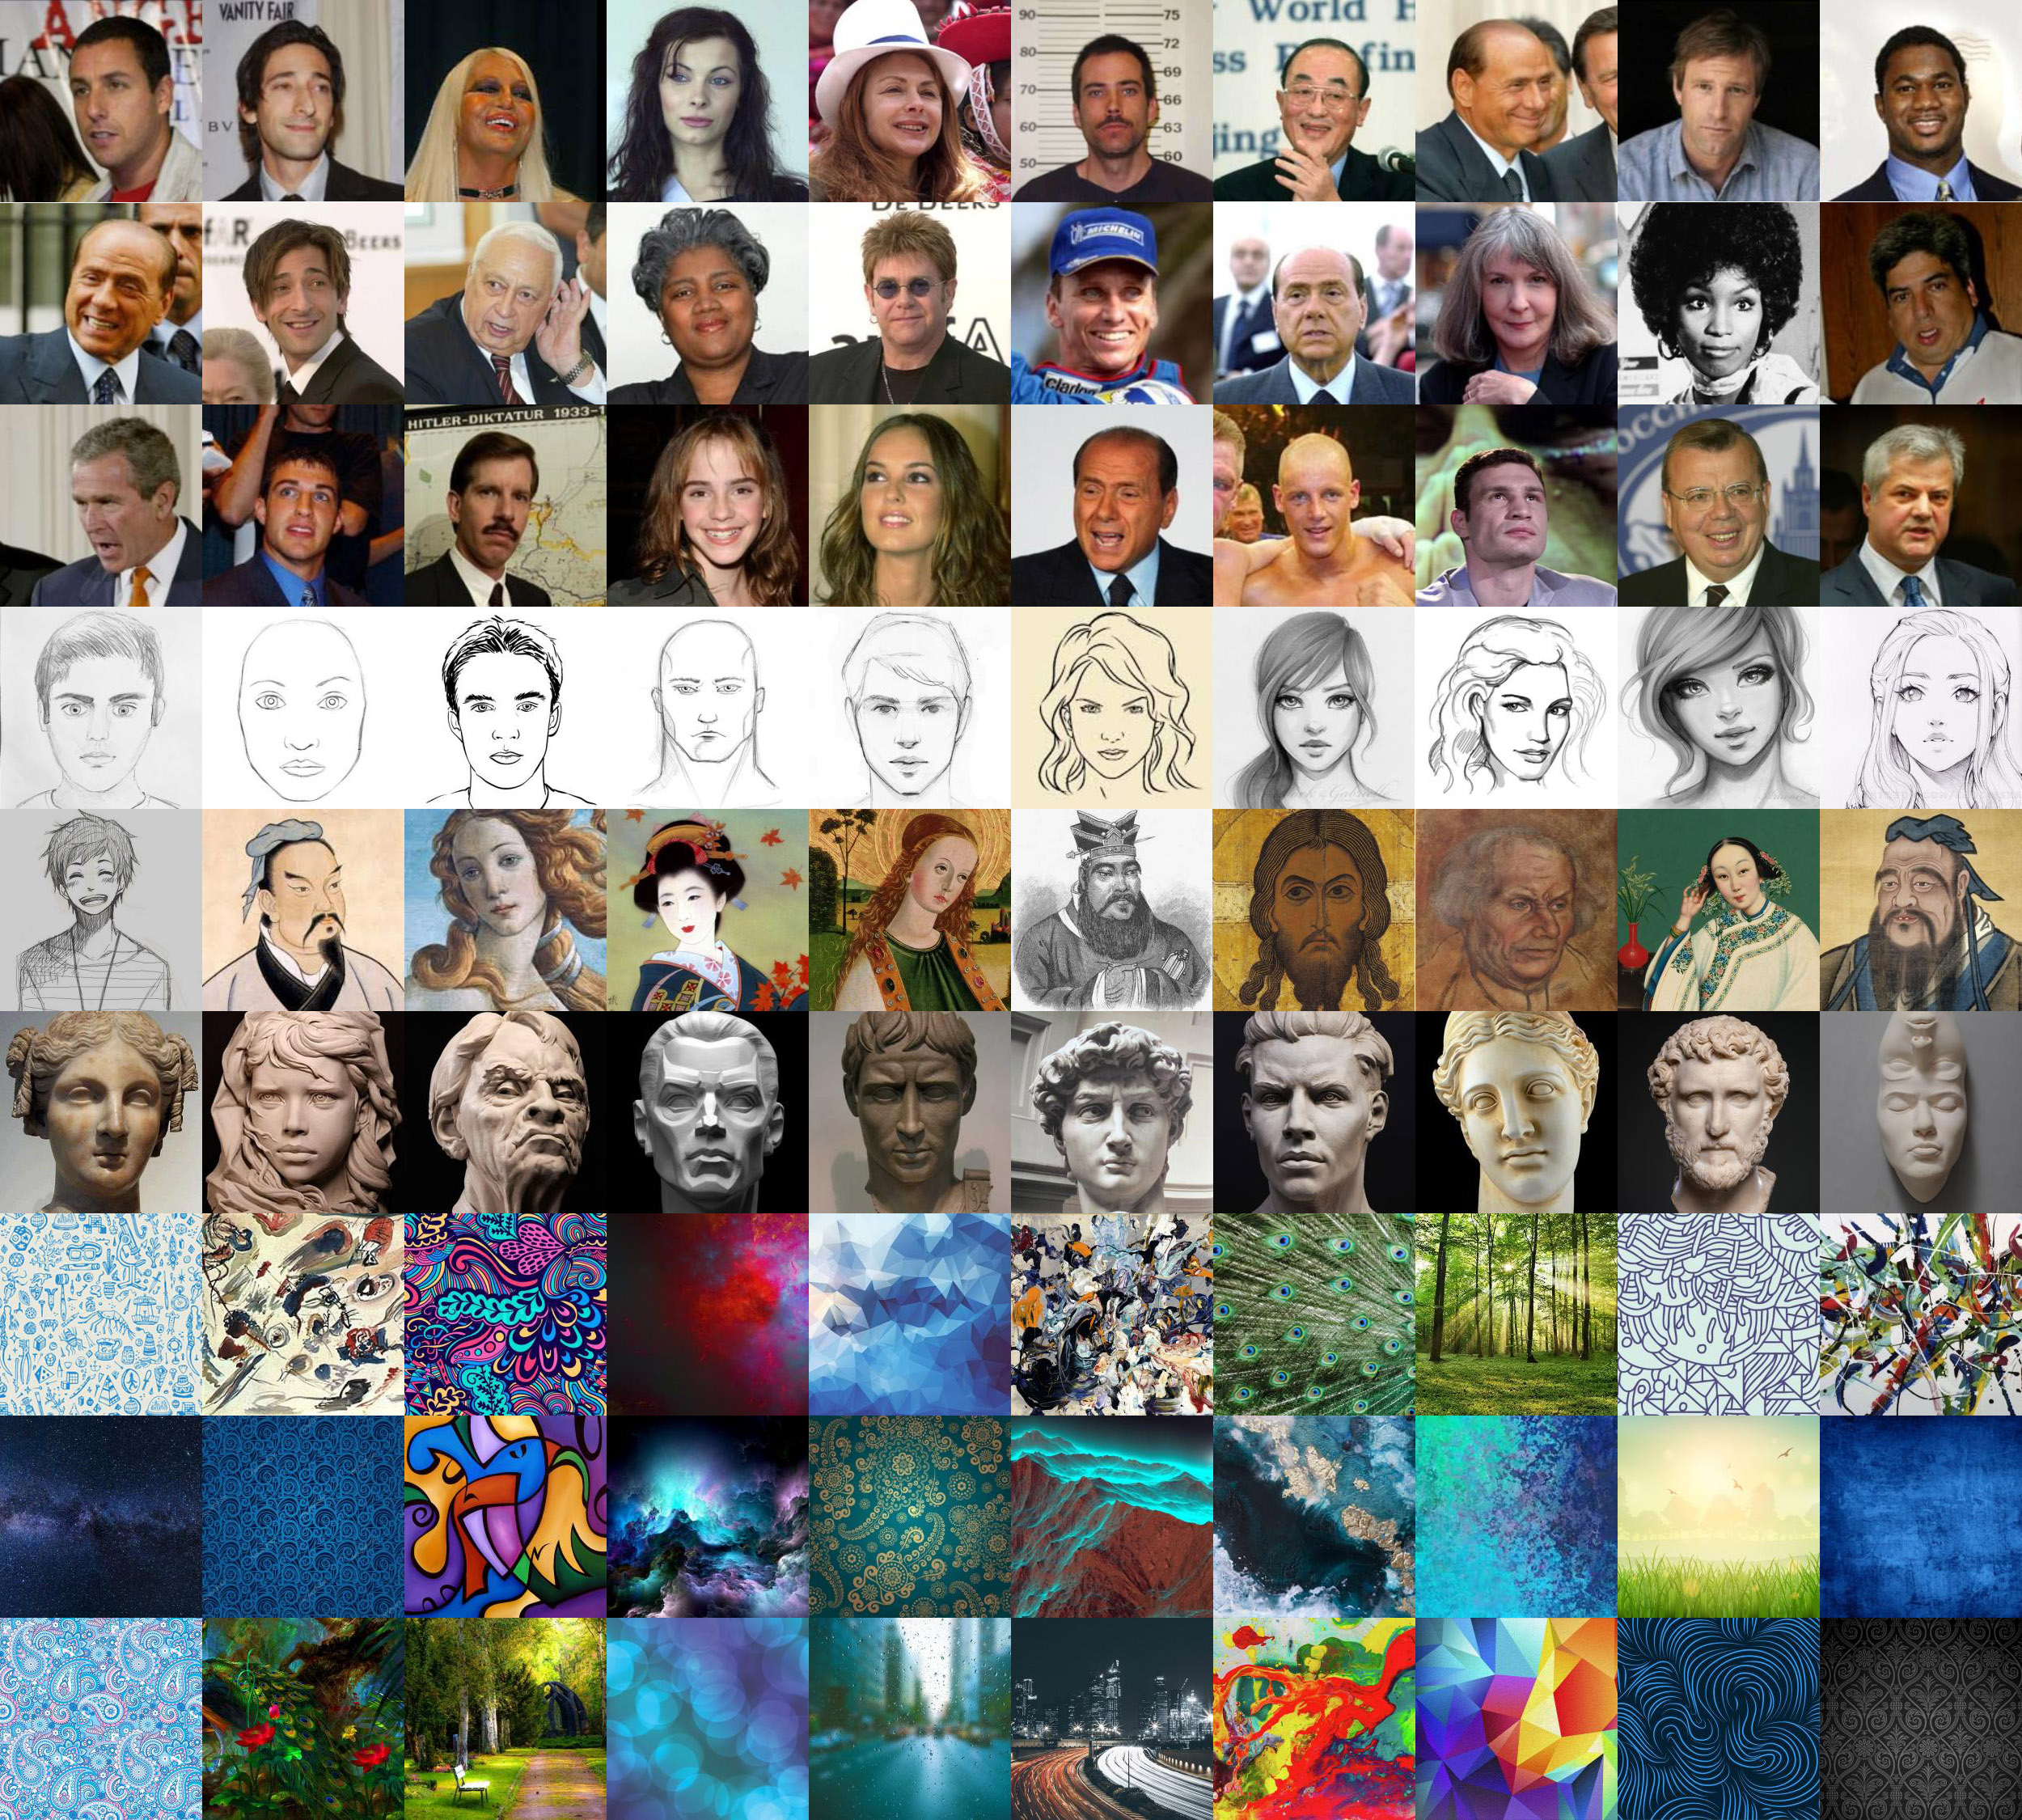
\includegraphics[width=14cm]{emp_studies/fd_dataset}
	%	\caption{Dataset for the Experiment 1}
	%	\label{fig:fd_dataset}
	%\end{figure}

	\subsection{Results}
	The results of the experiment are shown in the Table \ref{table:experiment_1_res}, where the rows refer to the prediction of the classifier and the columns refer to the three different datasets (in the case of the near-face dataset, each sub-group is shown in a different column).

	\begin{table}[H]
		\centering
		\resizebox{\textwidth}{!}
		{		
		    \begin{tabular}{L{3.5cm} | R{2.7cm} | R{0.9cm} | R{0.9cm} | R{0.9cm} | R{2.7cm} |}
			    \cline{2-6}
			    & \multicolumn{1}{c|}{Face dataset} & \multicolumn{3}{c|}{Near-face dataset} & \multicolumn{1}{c|}{Non-face dataset} \\ 
			    \hline
			    \multicolumn{1}{|c|}{Face detected} 	& 27 		& 6 & 6 & 10 		&  0 \\
				\hline
				\multicolumn{1}{|c|}{Face not detected} &  3 		& 5 & 3 &  0 		& 30 \\
				\hline
			\end{tabular}
		}
		\caption{Results of the Experiment 1}
	    \label{table:experiment_1_res}
	\end{table}

	% Look up confusion matrix, precision and recall
	\subsection{Evaluation}

\section{Effectiveness of Convolutional Neural Networks for Face Recognition}
	\subsection{Objective}
	%How many faces are correctly recognised?
	%How many faces are missed (false negatives)?
	\subsection{Method and parameters}
	%50 images of Mario: different illumination, pose, rotation, scale.
	\subsection{Data set}
	\subsection{Results}
	% Look up confusion matrix, precision and recall
	\subsection{Evaluation}




\chapter{Discussion and Conclusion}
\label{ch:conclussions}
In this section we will discuss how the objectives of this report, indicated at the beginning, have been achieved. A brief section about further work on the project is included at the end.

First of all, the development of the \textit{Intelligent Assistant} has been a complete success. The application combine the lightweight architecture of a Raspberry Pi and the computing power of a usual computer thanks to a client-server communication. The Raspberry Pi runs a graphical user interface (\gls{gui}) that allow users to take a photo of themselves and send it to the server via HTTP. The server, created using the micro-framework Flask, receives this photo and apply a face detection pre-processing using Viola-Jones Haar cascades and then the face recognition process with a \gls{cnn} using the library Tensorflow.

Once the user is recognised, the next class of the student in the day is obtained using web scraping from \textit{timetable.ul.ie}. The map from the actual location of the student to that class is obtained just after, showing all this information in the \gls{gui} to be accessible to the user. All the intermediate situations, such as when the student's face is not detected or recognised, or when the student has no more classes in the day, have been covered. 


\bibliographystyle{agsm}
\bibliography{ref}  

\begin{appendices}
\chapter{Application icons}
\label{ch:appendix_a}

\begin{figure*}[h!t]
	\centering
	\begin{multicols}{4}
		\hspace{\linewidth} 
	    
\includegraphics[width=3.15cm]{app_icons/play_button.png}\par 
	    
\includegraphics[width=3.15cm]{app_icons/play_button_fill_blue.png}\par 
	    \hspace{\linewidth}
    \end{multicols}
	\caption{Play icons from the Home window}
\end{figure*}

\begin{figure*}[h!t]
	\centering
	
\includegraphics[width=4cm]{app_icons/red_cross.png}
	\caption{Red cross icon from the Error Window}
\end{figure*}

\begin{figure*}[h!t]
	\centering
	\begin{multicols}{4}
		\hspace{\linewidth} 
	    
\includegraphics[width=3.15cm]{app_icons/home.png}\par 
	    
\includegraphics[width=3.15cm]{app_icons/home_blue.png}\par 
	    \hspace{\linewidth}
    \end{multicols}
	\caption{Home icons from the lateral menu}
\end{figure*}


\begin{figure*}[h!t]
	\centering
	\begin{multicols}{4}
		\hspace{\linewidth} 
	    
\includegraphics[width=3.15cm]{app_icons/camera.png}\par 
	    
\includegraphics[width=3.15cm]{app_icons/camera_blue.png}\par 
	    \hspace{\linewidth}
    \end{multicols}
	\caption{Camera icons from the lateral menu}
\end{figure*}

\begin{figure*}[h!t]
	\centering
	\begin{multicols}{4}
		\hspace{\linewidth} 
	    
\includegraphics[width=3.15cm]{app_icons/timetable_ready.png}\par 
	    
\includegraphics[width=3.15cm]{app_icons/timetable_ready_blue.png}\par 
	    \hspace{\linewidth}
    \end{multicols}

	\begin{multicols}{4}
		\hspace{\linewidth} 
	    
\includegraphics[width=3.15cm]{app_icons/timetable_waiting.png}\par 
	    
\includegraphics[width=3.15cm]{app_icons/timetable_waiting_yellow.png}\par 
	    \hspace{\linewidth}
    \end{multicols}

    
\includegraphics[width=3.15cm]{app_icons/timetable_not_ready.png}

	\caption{Timetable icons from the lateral menu}
\end{figure*}

\begin{figure*}[h!t]
	\centering
	\begin{multicols}{4}
		\hspace{\linewidth} 
	    
\includegraphics[width=3.15cm]{app_icons/user_waiting.png}\par 
	    
\includegraphics[width=3.15cm]{app_icons/user_not_ready.png}\par 
	    \hspace{\linewidth}
    \end{multicols}
	\caption{User icons from lateral menu}
\end{figure*}

\begin{figure*}[h!t]
	\centering
	\begin{multicols}{4}
		\hspace{\linewidth} 
	    
\includegraphics[width=3.15cm]{app_icons/map_ready.png}\par 
	    
\includegraphics[width=3.15cm]{app_icons/map_ready_blue.png}\par 
	    \hspace{\linewidth}
    \end{multicols}

	\begin{multicols}{4}
		\hspace{\linewidth} 
	    
\includegraphics[width=3.15cm]{app_icons/map_waiting.png}\par 
	    
\includegraphics[width=3.15cm]{app_icons/map_waiting_yellow.png}\par 
	    \hspace{\linewidth}
    \end{multicols}

    
\includegraphics[width=3.15cm]{app_icons/map_not_ready.png}

	\caption{Map icons from the lateral menu}
\end{figure*}


\end{appendices}

\end{document}   
